\documentclass[12pt,a4paper,utf8]{ctexart}
\usepackage{ctex,amsmath,amssymb,subfig,cite,graphicx,diagbox,fontspec,fancyhdr,geometry}
\usepackage[ntheorem]{empheq}
\usepackage{enumitem,fullpage,cleveref,cellspace,listings,color,framed}
\definecolor{gray}{rgb}{0.5,0.5,0.5}
\definecolor{dkgreen}{rgb}{.068,.578,.068}
\definecolor{dkpurple}{rgb}{.320,.064,.680}

%set Fortran styles
\lstset{
    frameround=tftf,
    language=Fortran,
    keywords={SELECT,PROGRAM,PRINT,STOP,END,WRITE,INTEGER,REAL,COMPLEX,CHARACTER,LOGICAL,READ,FORMAT,IMPLICIT,PARAMETER,DATA,EQUIVALENCE,TYPE,PAUSE,CONTINUE,CYCLE,EXIT,IF,SELECT,DO,ALLOCATE,DEALLOCATE,WHERE,FORALL,SUBROUTIHNE,CALL,RETURN,FUNCTION,COMMON,BLOCK DATA,SAVE,INTERFACE,CONTAIN,MODULE,USE,PUBLIC,PRIVATE,ENTRY,OPEN,INQUIRE,CLOSE,NAMELIST,POINTER,NULLFY,REWIND,BACKSPACE,ENDFILE
    },
    basicstyle=\small\ttfamily,
    numbers=left,
    numberstyle=\small,
    keywordstyle=\color{blue}\bfseries,
    commentstyle=\color{dkgreen},
    stringstyle=\color{dkpurple},
    backgroundcolor=\color{white},
    tabsize=2,
    showspaces=false,
    showstringspaces=false,
    breaklines=true,
    frame=trBL,
}
\CTEXsetup[format+={\raggedright}]{section}
\setlength{\parindent}{2em}
\geometry{
    textwidth=138mm,
    textheight=215mm,
    left=27mm,
    right=27mm,
    top=25.4mm,
    bottom=25.4mm,
    headheight=2.17cm,
    headsep=4mm,
    footskip=12mm,
    heightrounded,
}
\pagestyle{fancy}
\lhead{\textsl{2021秋-计算物理A}}
\chead{}
\rhead{\textsl{PB19020634-于浩然}}
\lfoot{}
\cfoot{\thepage}
\rfoot{}

\begin{document}
\begin{center}
    {\LARGE\textbf{计算物理作业十六}}\\
    \textrm{于浩然}~~~~~~\textrm{PB19020634}~~~~~~\textrm{2021.12.23}
\end{center}
\section{作业题目}

进行单中心DLA模型的模拟(可以用圆形边界,也可以用正方形边界),并用两种方法计算模拟
得到的DLA图形的分形维数,求分形维数时需要作出双对数图.

\section{算法简介}
\subsection{DLA模型}

\textbf{DLA(扩散限制聚集)}模型是一种著名的二维随机生长图形。要产生这一图形,则需要:
\begin{itemize}
    \item
        首先在二维正方格子的中心放一个粒子作为核心,再在远处随机产生一个粒子使其做
        随机扩散运动;
    \item
        当粒子运动到已存在粒子周围的八个格子中时,停止随机扩散,粒子成为核心的一部分;
    \item
        在远处不断产生新的粒子重复上述过程,直到成千上万个粒子聚集成为分叉状的
        DLA生长图形.
\end{itemize}

\subsection{盒计数法求分形维数}
    将一定尺寸(边长为$\varepsilon$)的网格覆盖在分形图形上,计数网格中有图形像素的
    方格数目$N(\varepsilon)$,直至网格尺寸达到像素大小为止.
    为减少误差,应当使不同尺寸的网格能覆盖相同大小的图形. 
    作$\ln N(\varepsilon)\sim
    \ln(1/\varepsilon)$图,若得到一条直线,则直线的斜率$D$即为图形的分维.

\subsection{Sandbox法求分形维数}
    Sandbox法即为将一系列尺寸$r(r>1)$的不断增大的方框(或圆)覆盖到分形图形上,计数
    不同方框(或圆)中像素数$N$. 作$\ln N \sim \ln
    r$图,则直线部分的斜率即为分形维数$D$.

\section{编程实现}

用Fortran90编写程序,分别在三个子程序中实现DLA模型的生成、盒子计数法求分维、
Sandbox法求分维,并装在一个模块 \texttt{MODULE DLA}中. 

\begin{itemize}
    \item \texttt{SUBROUTINE Generator(particles, steps, r0, rmax, resc,
        filename)}

        基于随机数生成DLA图形的子程序.
        使用两组随机数,如下:
        \begin{itemize}
            \item \texttt{rand0} 

                数组大小和粒子数
                \texttt{particles}相同,用于生成每个粒子的初始位置.
            \item \texttt{rand}

                数组大小和预计最大步数 \texttt{steps}相同,用于决定每一次
                随机行走的方向,具体实现见函数 \texttt{FUNCTION walk(dir)}.
        \end{itemize}
        还有一个算法用于验证粒子是否已经运动到已存在粒子的附近:
        \begin{itemize}
            \item 首先有一个用于记录网格占据状态的网格矩阵(数组) \texttt{lattice},
                当网格上某处有已存在的粒子则在此处 \texttt{lattice=1}.
                粒子当前位置的坐标为$(x, y)$(二维数组),对网格矩阵的切片 
                \texttt{lattice(x-1:x+1,
                y-1:y+1)}求和:若求和不为零,说明周围已经存在其他粒子,停止模拟.
        \end{itemize}
    具体取参数为: 模拟的总粒子数 \texttt{particles=100000};预计最大步数
    \texttt{steps=500000},当粒子超过这一步数还没有结合是死亡;初始随机点
    与中心点固定距离 \texttt{r0 = 400},点会在这一半径的圆周上随机生成;
    结合图形的边界取为正方形框,其边长的一半为
    \texttt{rmax = 256};粒子逃逸距离 \texttt{resc=450},当粒子的横坐标或
    纵坐标值比 \texttt{resc}大时,粒子死亡.
    
\item \texttt{SUBROUTINE Box(resc, rmax, filename)}

    读取前面子程序中生成的大小为(-450:450, -450:450)的 \texttt{lattice}矩阵,
    为简化取网格步骤取其(-255:256, -255:256)部分. 取$\varepsilon=2^k$,容易得到
    各$\varepsilon$值对应的$N(\varepsilon)$.

\item \texttt{SUBROUTINE Sandbox(resc, rmax, filename)}

    与上面的子程序同理,取$r=2^k$.
\end{itemize}

\newpage
\section{计算结果}

\subsection{DLA生长图形}
将计算所得的DLA模型绘制散点图展示如下:
\begin{figure}[!h]
    \centering
    \subfloat[]{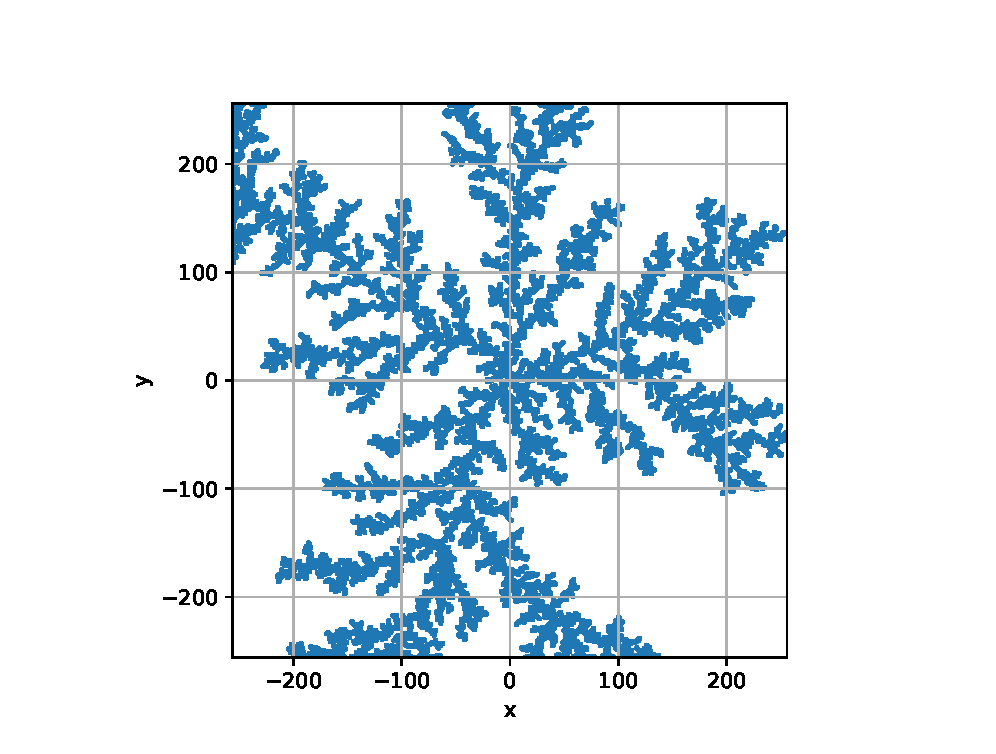
\includegraphics[width=0.8\textwidth]{plain.eps}}
    \hfill
    \subfloat[]{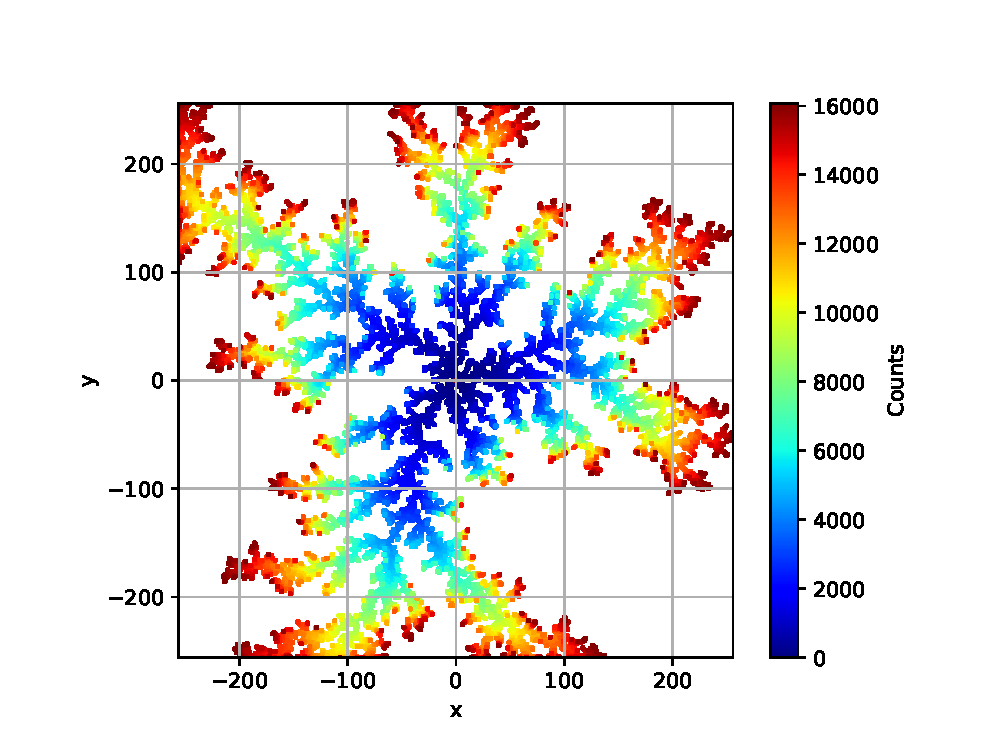
\includegraphics[width=0.8\textwidth]{color.eps}}
    \caption{DLA生长模型$(r=256pxs)$}
\end{figure}

图1(a)清晰地展示了DLA图形的枝杈状结构,而在图1(b)中展示了点生成的先后顺序.

\subsection{盒子计数法求分维}

作图并显示拟合直线及其信息:
\begin{figure}[!h]
    \centering
    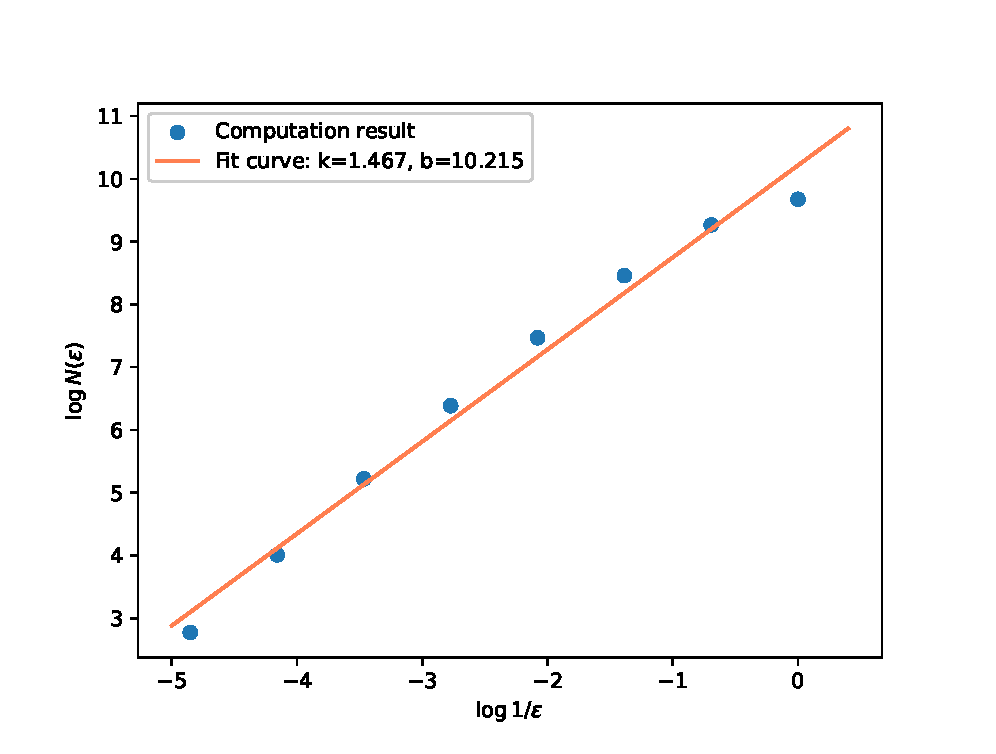
\includegraphics[width=0.6\textwidth]{box.eps}
    \caption{盒计数法拟合曲线}
\end{figure}

由直线斜率可知:所得DLA图形的分维为$D=1.467$.
\subsection{Sandbox法求分维}

作图并显示拟合直线及其信息:
\begin{figure}[!h]
    \centering
    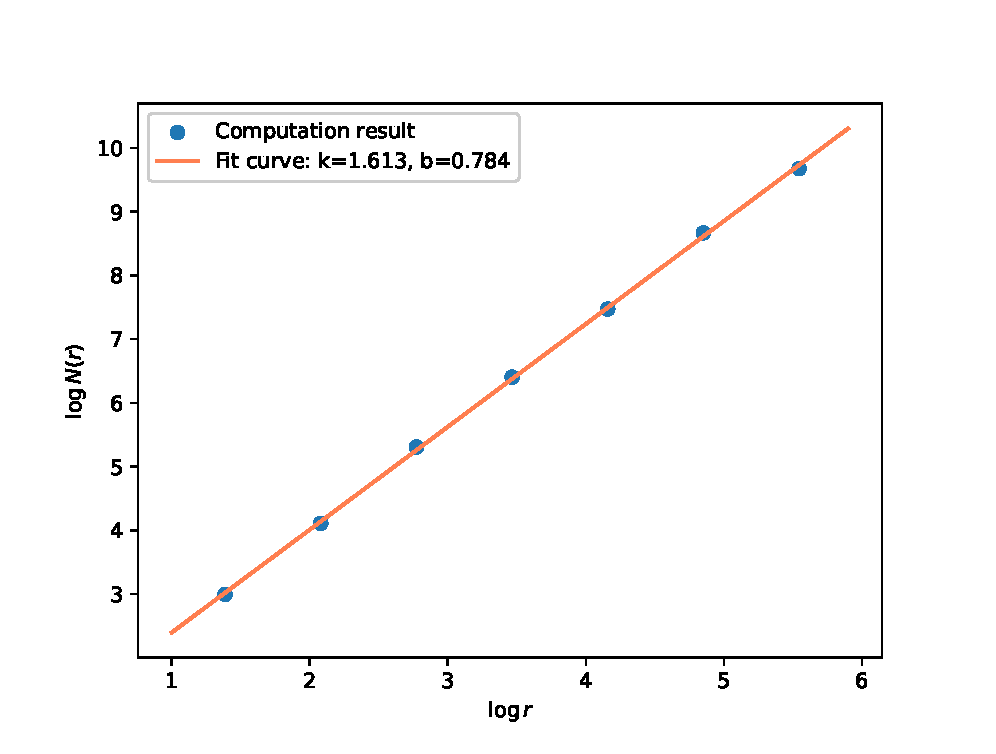
\includegraphics[width=0.6\textwidth]{sand.eps}
    \caption{Sandbox法拟合曲线}
\end{figure}

由直线斜率可知,所得DLA图形的分维为$D=1.613$.

\section{结论}

从所作的图像可看出直线拟合的非常好,得到了比较合理的结果. 
计算所得的分维由于计算方法不同而存在一定差异,这可能随着
模拟点的进一步增多而逐渐消失. 

本次作业实现了DLA模型的模拟,进一步实践了随机行走的运用,并计算了其分维以更好地了解分形
的性质.

\section{源代码}
\subsection{Fortran90代码}
\begin{framed}
\begin{lstlisting}[language=Fortran]
MODULE DLA
IMPLICIT NONE
REAL(KIND=8) :: pi = 3.14159265358979
CONTAINS
SUBROUTINE Generator(particles, steps, r0, rmax, resc, filename) ! 生成DLA图形的子程序
    INTEGER(KIND=4), INTENT(IN) :: particles, steps, r0, rmax, resc
    INTEGER(KIND=4) :: i, j, dir, r(2), pos(0:particles, 2), recorded
    INTEGER(KIND=4), DIMENSION(-resc:resc, -resc:resc) :: lattice
    REAL(KIND=8) :: seed, rand0(particles), rand(steps)
    CHARACTER(LEN=*) :: filename

    CALL RANDOM_NUMBER(seed)
    CALL Schrage(particles, INT(2147483647 * seed), rand0)
    lattice = 0 ! 用来记录坐标对应网格的占有情况
    lattice(-1:1, -1:1) = 1 ! 设置原点初始占据
    pos(0, :) = [0, 0] ! 记录DLA图形上像素点的坐标
    recorded = 1
    DO i = 1, particles
        r(1) = INT(r0 * COS(2 * pi * rand0(i)))
        r(2) = INT(r0 * SIN(2 * pi * rand0(i)))
        ! 用一个随机数产生粒子开始随机行走的初始点

        CALL RANDOM_NUMBER(seed)
        CALL Schrage(steps, INT(2147483647 * seed), rand)
        ! 产生用于判断粒子运动方向的随机数序列
        DO j = 1, steps
            dir = INT(4 * rand(j)) ! 设dir=0,1,2,3分别对应左,下,右,上
            r = r + walk(dir) ! 粒子随机行走一步
            IF (ABS(r(1)) > resc .OR. ABS(r(2)) > resc) THEN
                EXIT ! 若大于逃逸距离则停止计算
            ENDIF
            IF (SUM(lattice((r(1) - 1):(r(1) + 1), (r(2) - 1):(r(2) + 1))) .NE. 0) THEN
                IF(ABS(r(1)) <= rmax .AND. ABS(r(2)) <= rmax) THEN
                    ! 如果点在正方形范围(-rmax:rmax, -rmax:rmax)内则记录
                    lattice(r(1), r(2)) = 1 
                    ! 若粒子附近的八个点不是完全空的,则停止随机扩散使其成为核心的一部分
                    pos(recorded, 1) = r(1)
                    pos(recorded, 2) = r(2)
                    print *, r(1), r(2), real(i) / particles * 100, '%'
                    ! 记录新添加到DLA图形上像素点的坐标
                    recorded = recorded + 1 ! 添加到DLA图形上的像素数+1
                END IF
                EXIT
            END IF
        END DO
    END DO
    OPEN (1, file=filename)
    DO i = 1, recorded
        WRITE (1, *) pos(i, :)
    END DO
    CLOSE (1)
    OPEN (1, file='lattice.dat')
    WRITE (1, *) ((lattice(i, j), j = -resc, resc), i = -resc, resc)
    CLOSE (1)
END SUBROUTINE Generator  

SUBROUTINE Sandbox(resc, rmax, filename)
    CHARACTER(LEN=*) :: filename
    INTEGER(KIND=4),INTENT(IN) :: resc, rmax
    INTEGER(KIND=4) :: i, j, k, N(2:8), r(2:8)
    INTEGER(KIND=4) :: lattice(-resc:resc, -resc:resc), mesh(-rmax:rmax, -rmax:rmax)
    ! 读取Generator子程序中生成的格点占据矩阵
    OPEN (1, file='lattice.dat')
    READ (1, *) ((lattice(i, j), j = -resc, resc), i = -resc, resc)
    CLOSE (1)
    mesh = lattice(-rmax:rmax, -rmax:rmax) ! 取画出图像部分的像素点占据情况
    N = 0
    DO k = 2, 8
        r(k) = 2**k
        DO i = -r(k)+1, r(k)
            DO j = -r(k)+1, r(k)
                IF(lattice(i, j) .EQ. 1) THEN
                    N(k) = N(k) + 1 ! 当lattice值为1表示存在一个像素,N值累加
                END IF
            END DO
        END DO
    END DO
    OPEN (1, file=filename)
    DO k = 2, 8
        WRITE (1, *) r(k), N(k)
    END DO
    CLOSE (1)
END SUBROUTINE Sandbox

SUBROUTINE Box(resc, rmax, filename) ! 盒子计数法求分维子程序
    CHARACTER(LEN=*) :: filename
    INTEGER(KIND=4), INTENT(IN) :: resc, rmax
    INTEGER(KIND=4) :: i, j, k, N(0:7), eps(0:7)
    INTEGER(KIND=4) :: lattice(-resc:resc, -resc:resc), mesh(-rmax+1:rmax, -rmax+1:rmax)
    ! 读取Generator子程序中生成的格点占据矩阵
    OPEN (1, file='lattice.dat')
    READ (1, *) ((lattice(i, j), j = -resc, resc), i = -resc, resc)
    CLOSE (1)
    mesh = lattice(-rmax+1:rmax, -rmax+1:rmax) ! 取画出图像部分的像素点占据情况
    N = 0
    DO k = 0, 7
        eps(k) = 2**k
        DO i = -256 / eps(k), 256 / eps(k) 
            DO j = -256 / eps(k), 256 / eps(k)
                IF(SUM(lattice((i * eps(k) + 1):((i+1) * eps(k)), (j * eps(k) + 1):((j+1) * eps(k)))) .NE. 0) THEN
                    N(k) = N(k) + 1 ! 若网格中非空则盒子计数+1
                END IF
            END DO  
        END DO
    END DO
    OPEN (1, file=filename)
    DO k = 0, 7
        WRITE (1, *) eps(k), N(k)
    ENDDO
    CLOSE (1)
END SUBROUTINE Box

FUNCTION walk(direction) ! 将数字代号转换成位移坐标的函数
    INTEGER(KIND=4) :: direction
    INTEGER(KIND=4), DIMENSION(2) :: walk
    SELECTCASE(direction)
        CASE(0)
          walk = [-1, 0]
        CASE(1)
          walk = [0, -1]
        CASE(2)
          walk = [1, 0]
        CASE(3)
          walk = [0, 1]
    END SELECT
END FUNCTION walk
END MODULE DLA  

SUBROUTINE Schrage(num, z0, rand) 
    !Schrage随机数生成器子程序,将均匀随机数序列存放在数组rand中
    IMPLICIT NONE
    INTEGER(KIND=4) :: N = 1, num
    INTEGER :: m = 2147483647, a = 16807, q = 127773, r = 2836, In(num), z0
    REAL(KIND=8), INTENT(INOUT) :: rand(num)
    In(1) = z0 !将传入值z0作为种子
    rand(1) = REAL(In(1))/m
    DO N = 1, num - 1
        In(N + 1) = a * MOD(In(N), q) - r * INT(In(N) / q)
        IF (In(N + 1) < 0) THEN !若值小于零,按Schrage方法加m
            In(N + 1) = In(N + 1) + m
        END IF
        rand(N + 1) = REAL(In(N + 1))/m !得到第N+1个随机数
    END DO
END SUBROUTINE Schrage

PROGRAM MAIN
    USE DLA
    IMPLICIT NONE
    ! CALL Generator(100000, 500000, 400, 256, 450 ,'test.dat')
    CALL Box(450, 256, 'box.dat')
    ! CALL Sandbox(450, 256, 'sandbox.dat')
END PROGRAM MAIN
\end{lstlisting}
\end{framed}

\subsection{python绘图代码}
\begin{framed}
\begin{lstlisting}[language=python]
import numpy as np
import matplotlib.pyplot as plt
import matplotlib as mpl
import math

plt.rcParams['savefig.dpi'] = 300
plt.rcParams['figure.dpi'] = 300

dat = np.loadtxt('0_2.dat')
x = dat[0:100000]
y = dat[100001:200001]
plt.xlabel('x')
plt.ylabel('y')
plt.plot(x, y, linewidth=0.1)
plt.savefig('0_2.eps')
plt.show()
plt.scatter(x, y, c=range(100000), cmap=mpl.cm.jet, s=0.1)
plt.colorbar(label="Counts", orientation='vertical')
plt.xlabel('x')
plt.ylabel('y')
plt.savefig('0_2_1.eps')
plt.show()

dat = np.loadtxt('1_0.dat')
x = dat[0:100000]
y = dat[100001:200001]
plt.xlabel('x')
plt.ylabel('y')
plt.plot(x, y, linewidth=0.1)
plt.savefig('1_0.eps')
plt.show()
plt.scatter(x, y, c=range(100000), cmap=mpl.cm.jet, s=0.1)
plt.colorbar(label="Counts", orientation='vertical')
plt.xlabel('x')
plt.ylabel('y')
plt.savefig('1_0_1.eps')
plt.show()

dat = np.loadtxt('5_0.dat')
x = dat[0:100000]
y = dat[100001:200001]
plt.xlabel('x')
plt.ylabel('y')
plt.plot(x, y, linewidth=0.1)
plt.savefig('5_0.eps')
plt.show()
plt.scatter(x, y, c=range(100000), cmap=mpl.cm.jet, s=0.1)
plt.colorbar(label="Counts", orientation='vertical')
plt.xlabel('x')
plt.ylabel('y')
plt.savefig('5_0_1.eps')
plt.show()

\end{lstlisting}
\end{framed}
\end{document}
